Our initial focus centered on understanding and replicating the ABM presented in our selected paper. Therefore, we start by giving a concise summary of the relevant parts of this paper.

\subsection{Paper Summary}

The research paper \textit{Optimal Shepherding and Transport of a Flock} explores the techniques that a shepherd can employ to effectively guide a group of animals towards a specific destination. The investigation utilizes an ABM to simulate the behavior of both the shepherd and the flock, with the primary goal of maintaining flock cohesion while achieving the desired movement.

The paper identifies three distinct herding strategies, namely \textit{mustering}, \textit{droving}, and \textit{driving}. Mustering involves the shepherd circling the flock to keep it together, while droving entails the shepherd chasing the flock in the intended direction. Driving, on the other hand, involves the shepherd positioning themselves within the flock and guiding it from the inside. The paper delves into an analysis of the efficiency of these three strategies. The efficiency of a strategy is measured with respect to the three goals (A) moving the mass of the herd to the desired location, (B) not loosing any sheep in the process, and (C) keeping the target and the herd in alignment. 

The findings of the investigation suggest that the optimal herding strategy depends on just two parameters, namely the ratio of the herd size to the shepherd repulsion length and the ratio of herd speed to shepherd speed. The paper comes to the conclusion that droving is the most efficient strategy for managing small herds, while driving proves to be the most effective approach for cohesive, tightly-knit herds. Also, as the shepherd speed increases compared to the herd speed, the optimal strategy changes from droving to mustering.\\

Next, we executed the existing implementation of the ABM shared by our selected paper's authors in their GitHub repository\footnote{\url{https://github.com/arphysics/optimal-shepherding/tree/main/ABM_code}}. In the following subsection, we provide a detailed description of our procedure involved in running the model, along with the necessary steps to generate a plot and a video of the simulation results. All the following commands and actions were performed in a Linux operating system environment (Ubuntu 22.04.3).

\subsection{ABM recreation}

\subsubsection{Running the simulation}
The code of the ABM implementation can be found in the directory \texttt{ABM\_code}. The main file used for running the simulation is \texttt{simulate.cc}. The file \texttt{params.txt} contains the parameters for the simulation (e.g., amount of steps, speed of the herd). Since for the moment we are just focusing on recreating the model, we did not adjust any of these parameters yet. 

During the simulation process, the resulting data is recorded in two distinct output files, namely \texttt{data.txt} and \texttt{costdata.txt}. The former contains the positions of every agent and of the shepherd at each timestep and is the main data file for the simulation. The latter stores the values of the objective function at each timestep which is useful for analysis and debugging.

We successfully downloaded the implementation and executed the simulation by following these straightforward steps:

\begin{verbatim}
    git clone git@github.com:arphysics/optimal-shepherding.git
    cd optimal-shepherding/ABM_code
    cp ../paper_outputs/SI_ABM_videos/config.mk ..
    # replace g++-9 with g++-11 in ../config.mk
    make
    ./simulate
\end{verbatim}

\subsubsection{Creating a plot}
To visualize the simulation results with a plot, we employed the file \texttt{trajectory\_plotter.py} from the directory \texttt{ABM\_code}. The resulting plot is saved as \texttt{output\_plot.pdf}. We started by executing the following steps to run the plotting file:

\begin{verbatim}
    python3 -m pip install numpy Pillow pyparsing matplotlib
    python3 trajectory_plotter.py
\end{verbatim}

\noindent
This first attempt was unsuccessful as we encountered the following error:

\begin{Verbatim}[commandchars=\\\{\}]
\textcolor{red}{
    ValueError: setting an array element with a sequence. The requested array}
\textcolor{red}{
    would exceed the maximum number of dimension of 1.}
\end{Verbatim}

Upon careful inspection, we determined that the error stemmed from an attempt to modify two elements of a list simultaneously. It appears that this operation is not allowed when working with a Python list, but is feasible when using a NumPy array. Consequently, we adjusted the code at six specific locations in the way shown below.\\

\begin{tabular}{ll}
\textit{Initial code} & \texttt{xs[i] = [x[i], x[i] + unit\_perp[0] ]} \\
\textit{Updated version} & \texttt{xs[i] = np.array([x[i], x[i] + unit\_perp[0] ]).flatten()}
\end{tabular}\\

This solved the issue and we obtained the plot shown in figure \ref{fig:output_plot}.

\begin{figure}[h]
    \centering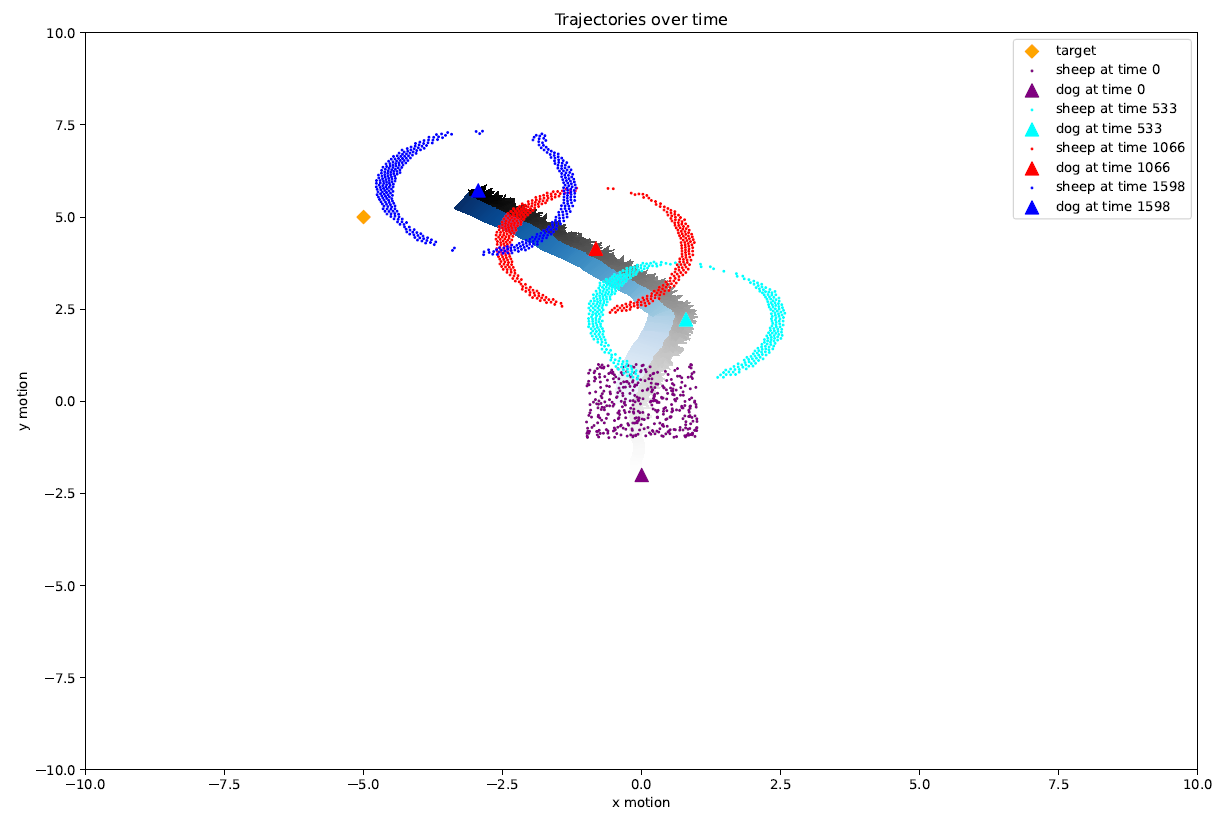
\includegraphics[width=0.9\textwidth]{figures/output_plot.png}\caption{Trajectory of the agents and the shepherd over time}
    \label{fig:output_plot}
\end{figure}

\subsubsection{Creating a video}
We also visualized the simulation results through a movie by using the file \texttt{newest\_visualizer.py} from the directory \texttt{ABM\_code}. The resulting video is saved as \texttt{output\_movie\_clone.mp4}. We performed the following steps to create a video of the results:

\begin{verbatim}
    mkdir test_plots
    sudo apt install -y ffmpeg
    python3 newest_visualizer.py
\end{verbatim}

We encountered the same error here as we did when creating the plot and were able to use the same solution to resolve it. The resulting video can be found in our GitHub repository\footnote{\url{https://github.com/ki-mberley/Collective-Behaviour/tree/main}}.
